\documentclass{article}
%==============================================================================%
%	                          Packages                                     %
%==============================================================================%
% Packages
\usepackage[utf8]{inputenc}
\usepackage{graphicx}
\usepackage{amsmath}
\usepackage{amssymb}
\usepackage{braket}
\usepackage[margin=0.7in]{geometry}
\usepackage[version=4]{mhchem}
\usepackage{url}
\usepackage{float}
%==============================================================================%
%                           User-Defined Commands                              %
%==============================================================================%
% User-Defined Commands
\newcommand{\be}{\begin{equation}}
\newcommand{\ee}{\end{equation}}
\newcommand{\benum}{\begin{enumerate}}
\newcommand{\eenum}{\end{enumerate}}
\newcommand{\pd}{\partial}
\newcommand{\dg}{\dagger}
%==============================================================================%
%                             Title Information                                %
%==============================================================================%
\title{Chem237: Lecture 6}
\date{4/12/18}
\author{Shane Flynn}
%==============================================================================%
%==============================================================================%
\begin{document}

\section*{Extreme Integration}
Start with Taylor Series.

If f(z) is regular in D, than all derivitives exist, therfore we can expand f(z) in a taylor series about some point z$_0$. 
\be
\begin{split}
    a &= f(z_0)\\
    a_n &= \frac{1}{n!} f^n(z_0)
\end{split}
\ee

The question is if the series converges?
If z$_0$ is in the center of a disk iwth radius r, such that r is equal to the distance between z$_0$ and teh closest singularity. 

\begin{figure}[H]
  \centering
    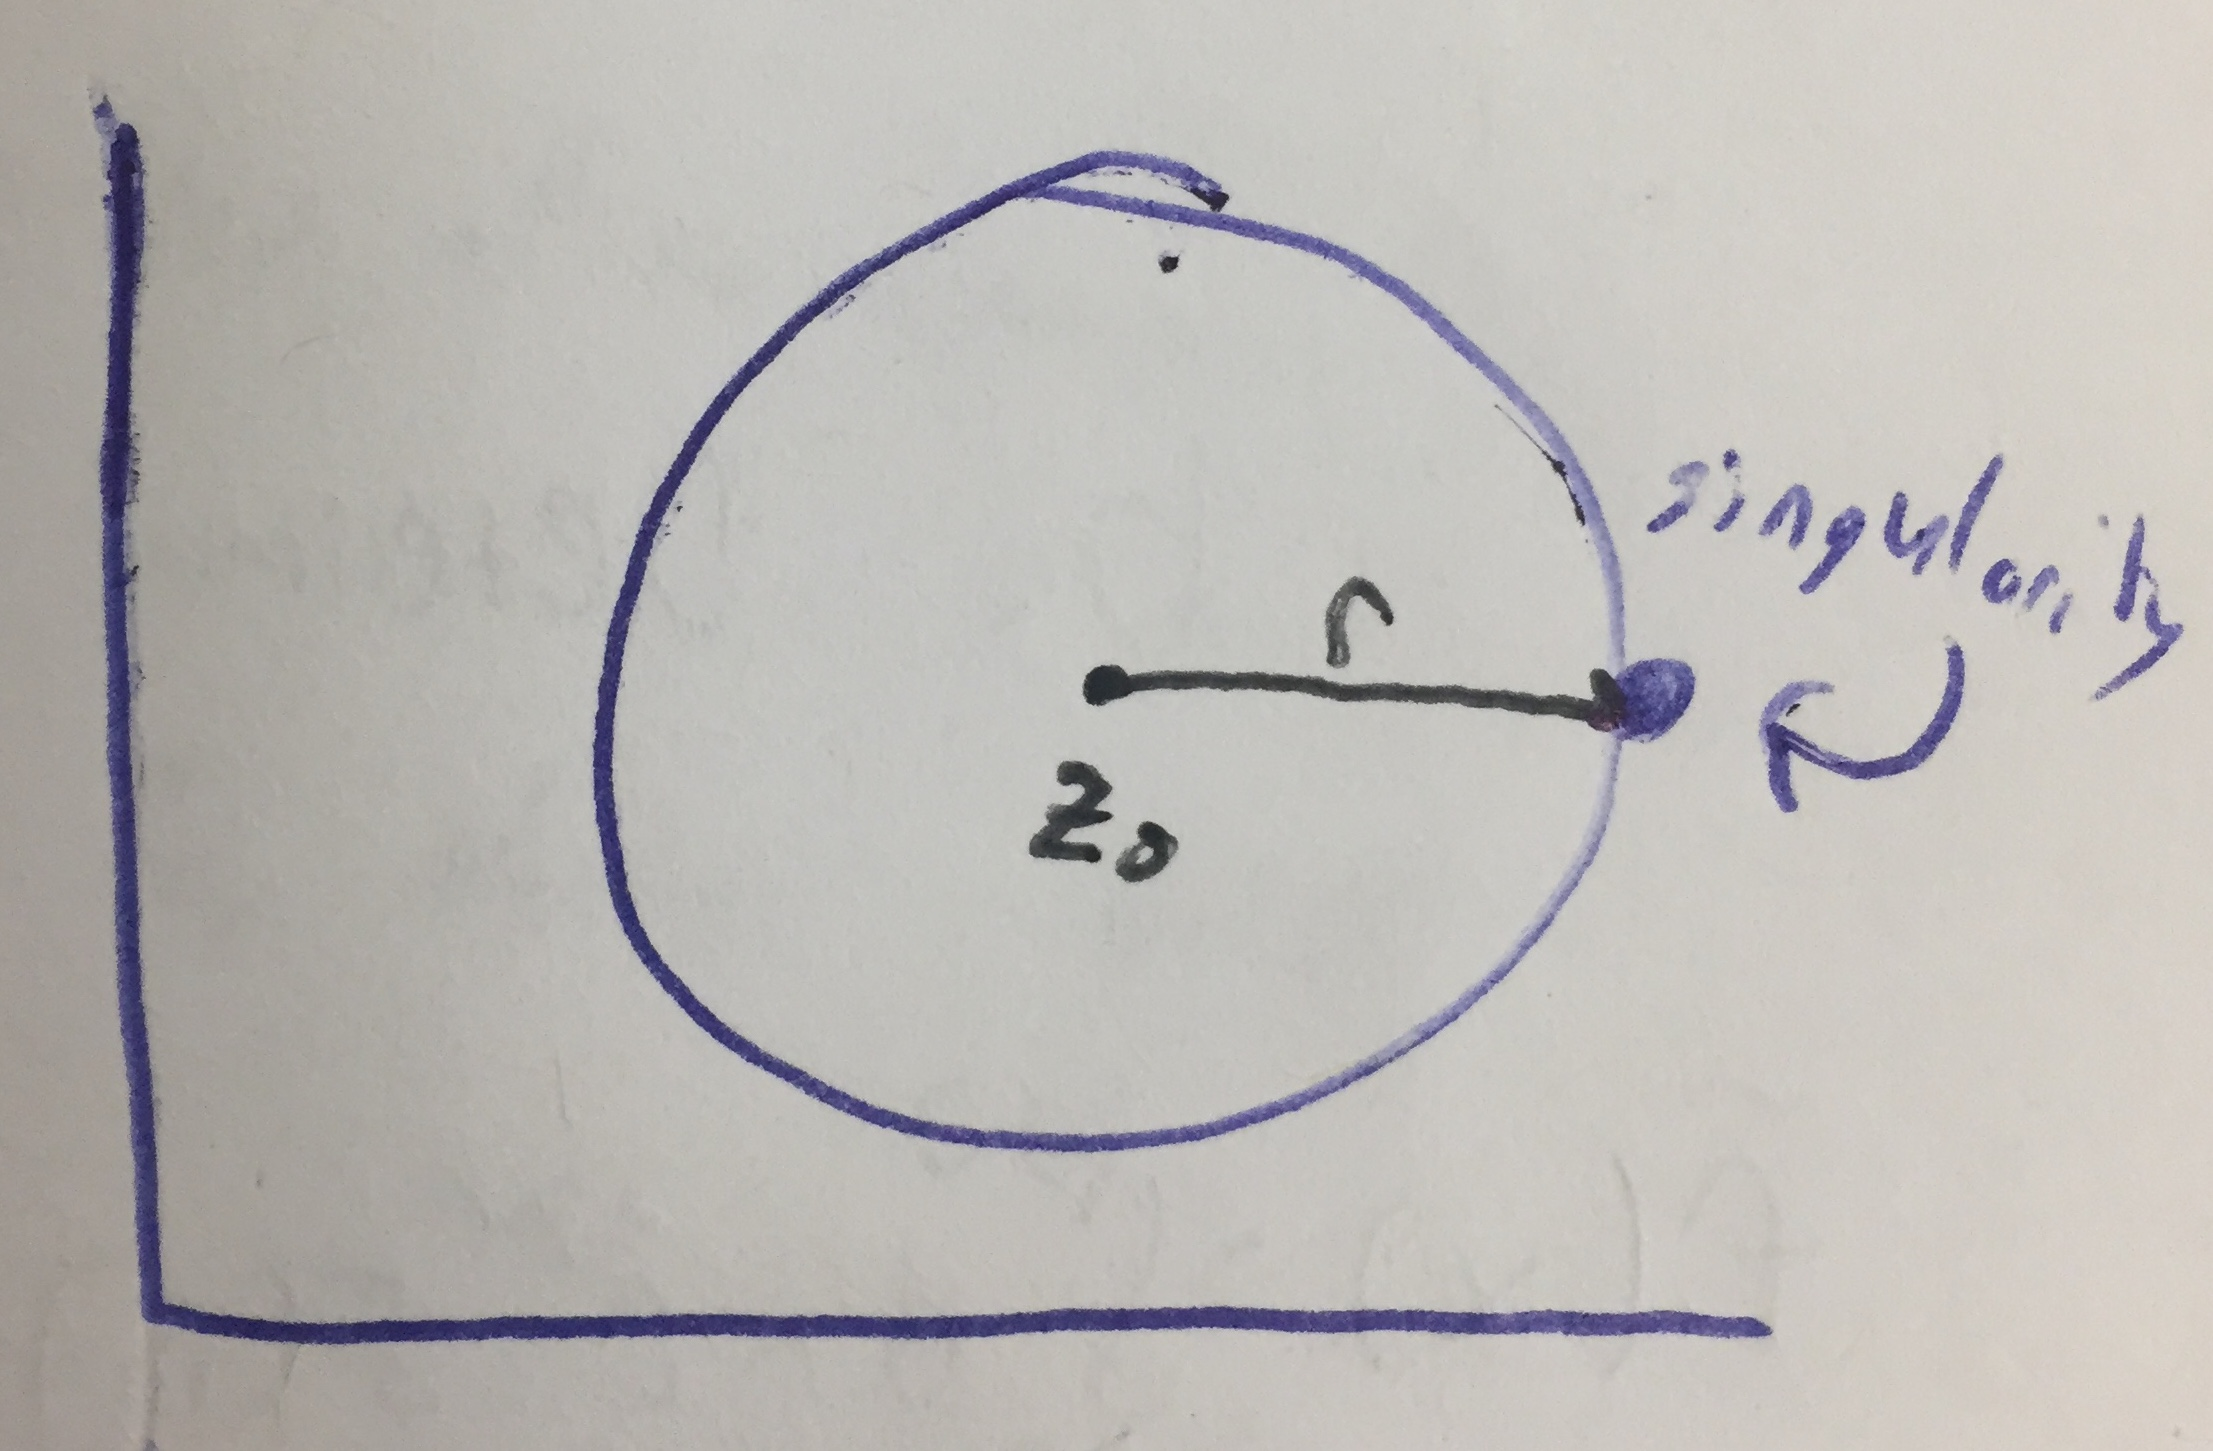
\includegraphics[scale=0.2]{Figures/converge.png}
    \caption{Make a caption. Radius of Convergence defined by r. R is length to closest singulaiity.}
\end{figure}

As an example consider 
\be
f(z) = \frac{1}{z}
\ee
The function exists everywhere, except for the singulairty at z=0. 
To evaluate we can expand the funciton
\be
\frac{1}{z} = \frac{1}{1-\left(\frac{z_0-z}{z_0}\right)^n}
\ee
We can now use a geometrix series
The Taylor series is
\be
\frac{1}{z_0} \sum_{n=0}^\infty \left(\frac{z_0-z}{z_o}\right)^n
\ee
To convege then 
\be
\frac{z-z_0}{z_0}< 1
\ee
We know z-z$_0 < z_0$. 

\subsection*{Laurent Series}
Expand the series about point z$_0$
\be
\begin{split}
    f(z) &= \sum_{n=-\infty}^\infty a_n (z-z_0)^n\\
    a_n &= \frac{1}{2\pi i} \oint_\gamma dz \frac{f(z)}{(z-z_0)^{n+1}}
\end{split}
\ee
Where teh second line comes from cauchy. 

As an example we can again use f(z) = $\frac{1}{z}$ whih is naturally the form for a laurentz series.
\be
\frac{1}{z} =\frac{a_1}{z-0}
\ee
Where we define a$_1$ = 1 and z$_0$ = 0

The contour would need to go around z$_0$, but we may not need to include z$_0$ in our domain (i.e. we can make the contour as small as we want around z$_0$ infinately small about the point. 
\begin{figure}[H]
  \centering
    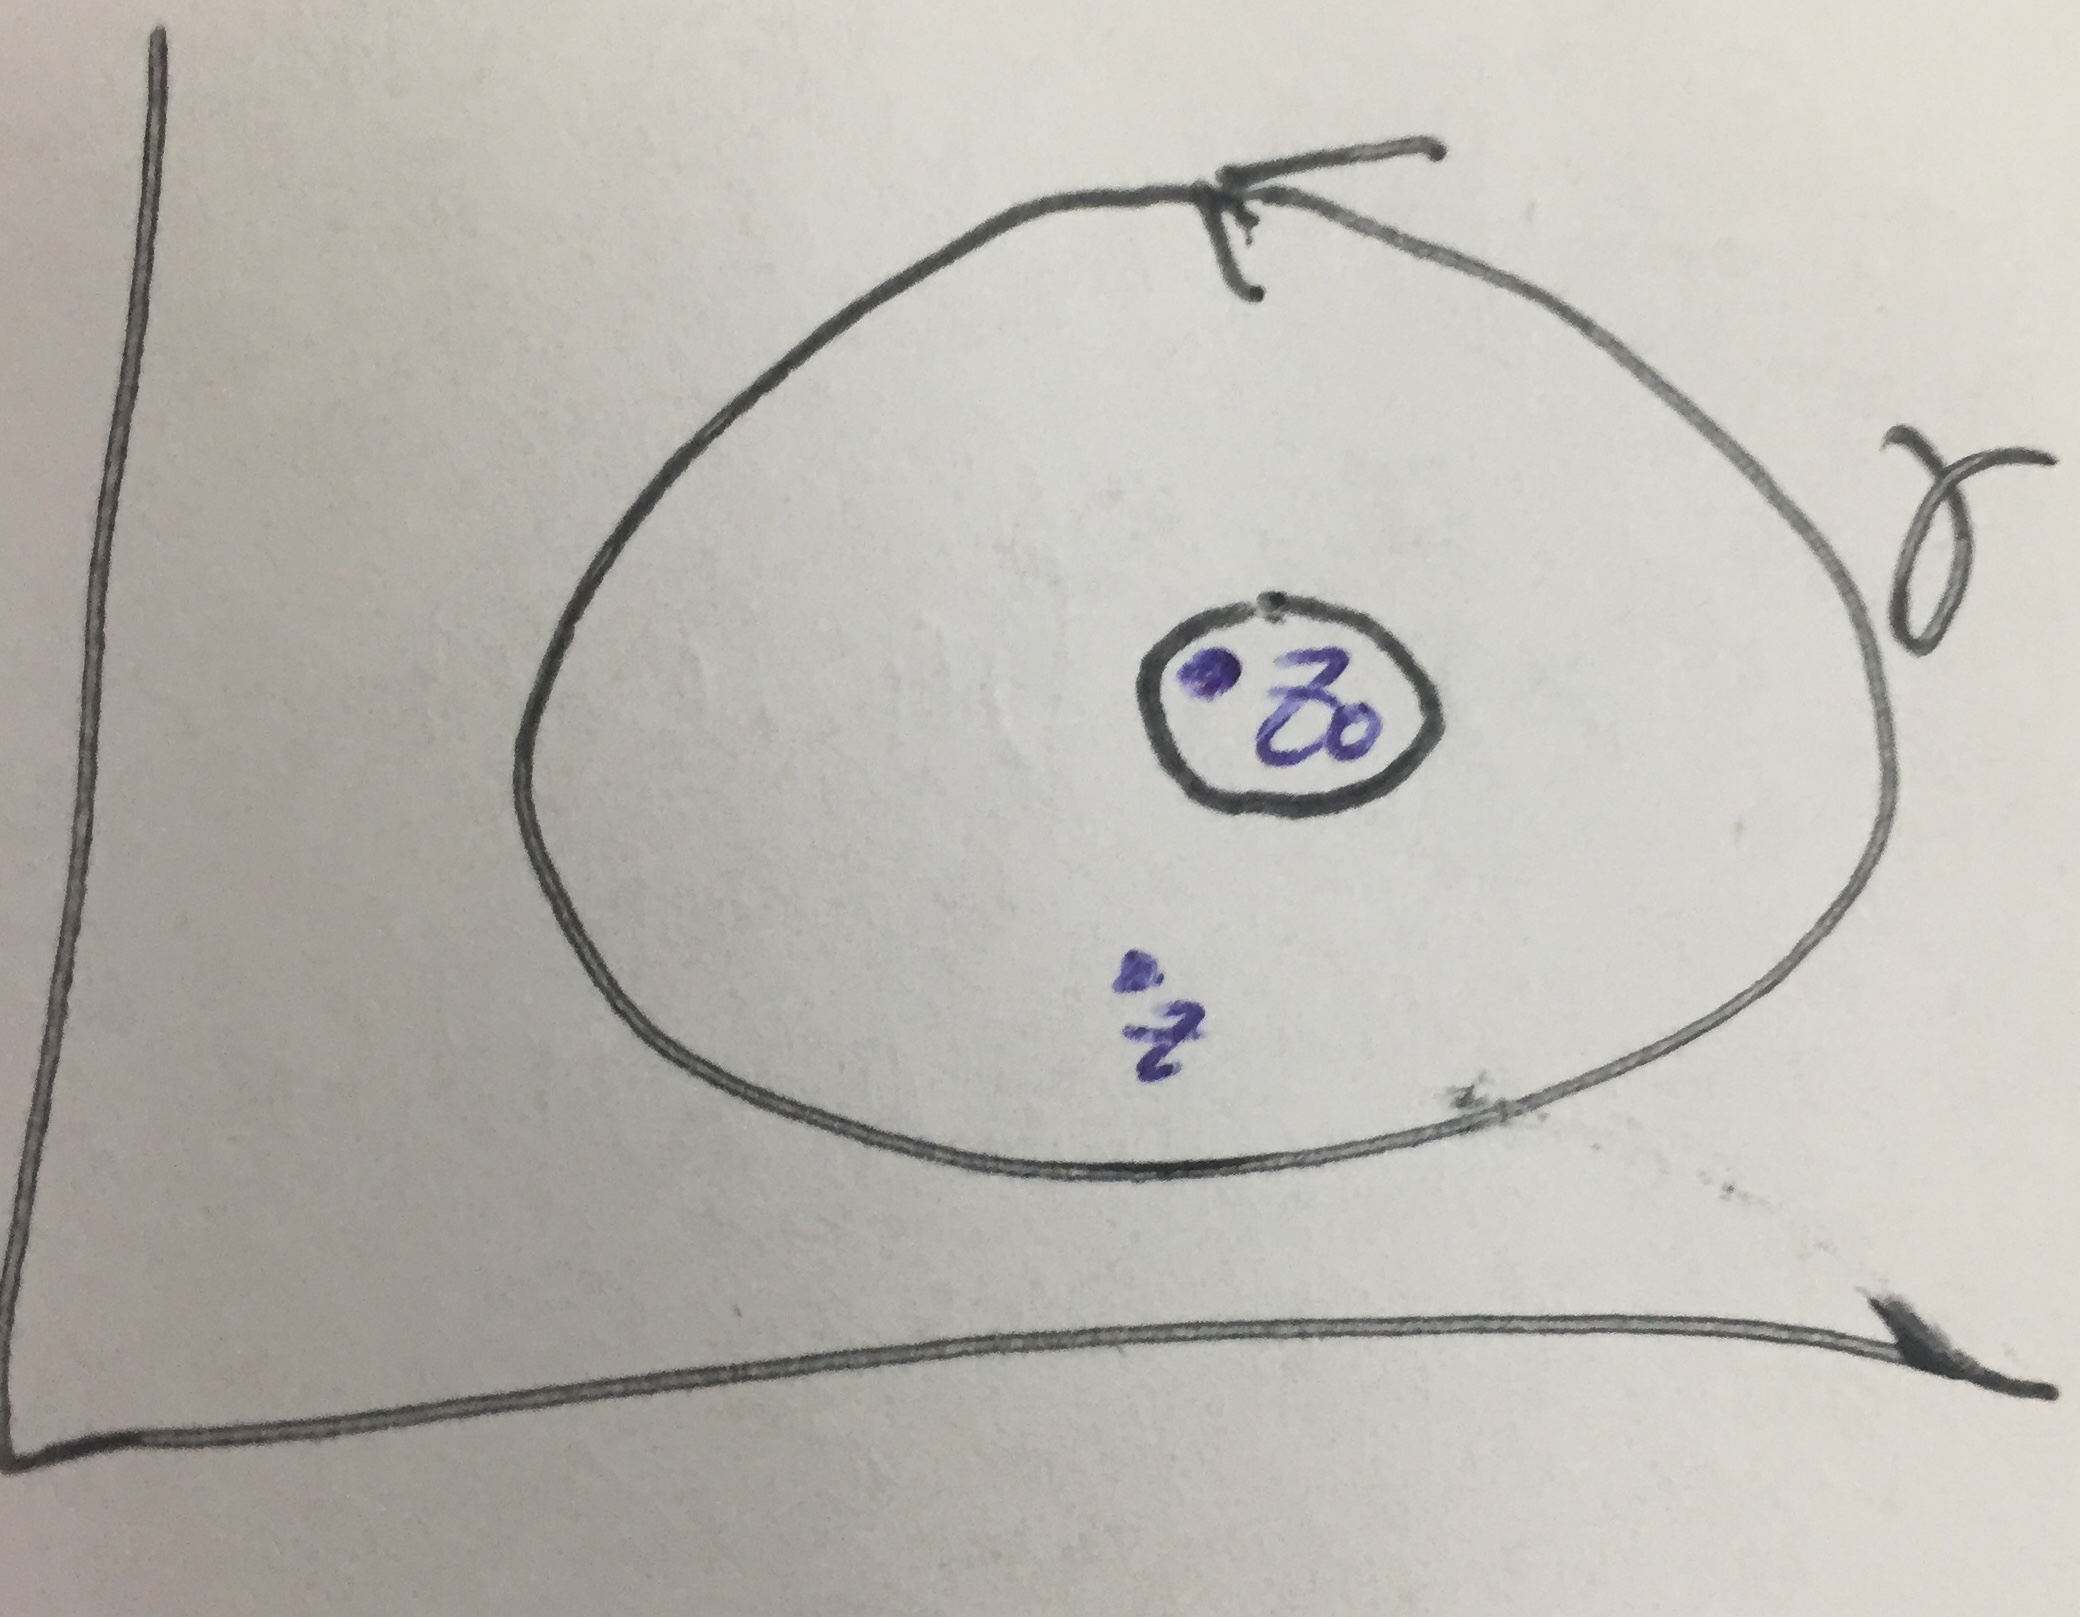
\includegraphics[scale=0.2]{Figures/laurent.png}
    \caption{Make a caption. Radius of Convergence defined by r. R is length to closest singulaiity.}
\end{figure}

We can now represent f(z) at any point z because the function is regular the integral is not a function of path. 

\subsection*{Pole}
z$_0$ is a simple pole of order M if a$_m \neq 0$, but for any m'$>$m a$_{m'}$=0.

If m is infinite, than z$_0$ is known as a essential singularity at this point. 

There are other types of singularities, ofr example  abranching point occurs for f(z) = $\sqrt{z}$. 
In polar coordinates we could write z = Re$^{i\theta}$. 
\be
    f(z) = \sqrt{z} = \sqrt{R}e^{i\theta}
    \ee
We can choose a new contour
\begin{figure}[H]
  \centering
    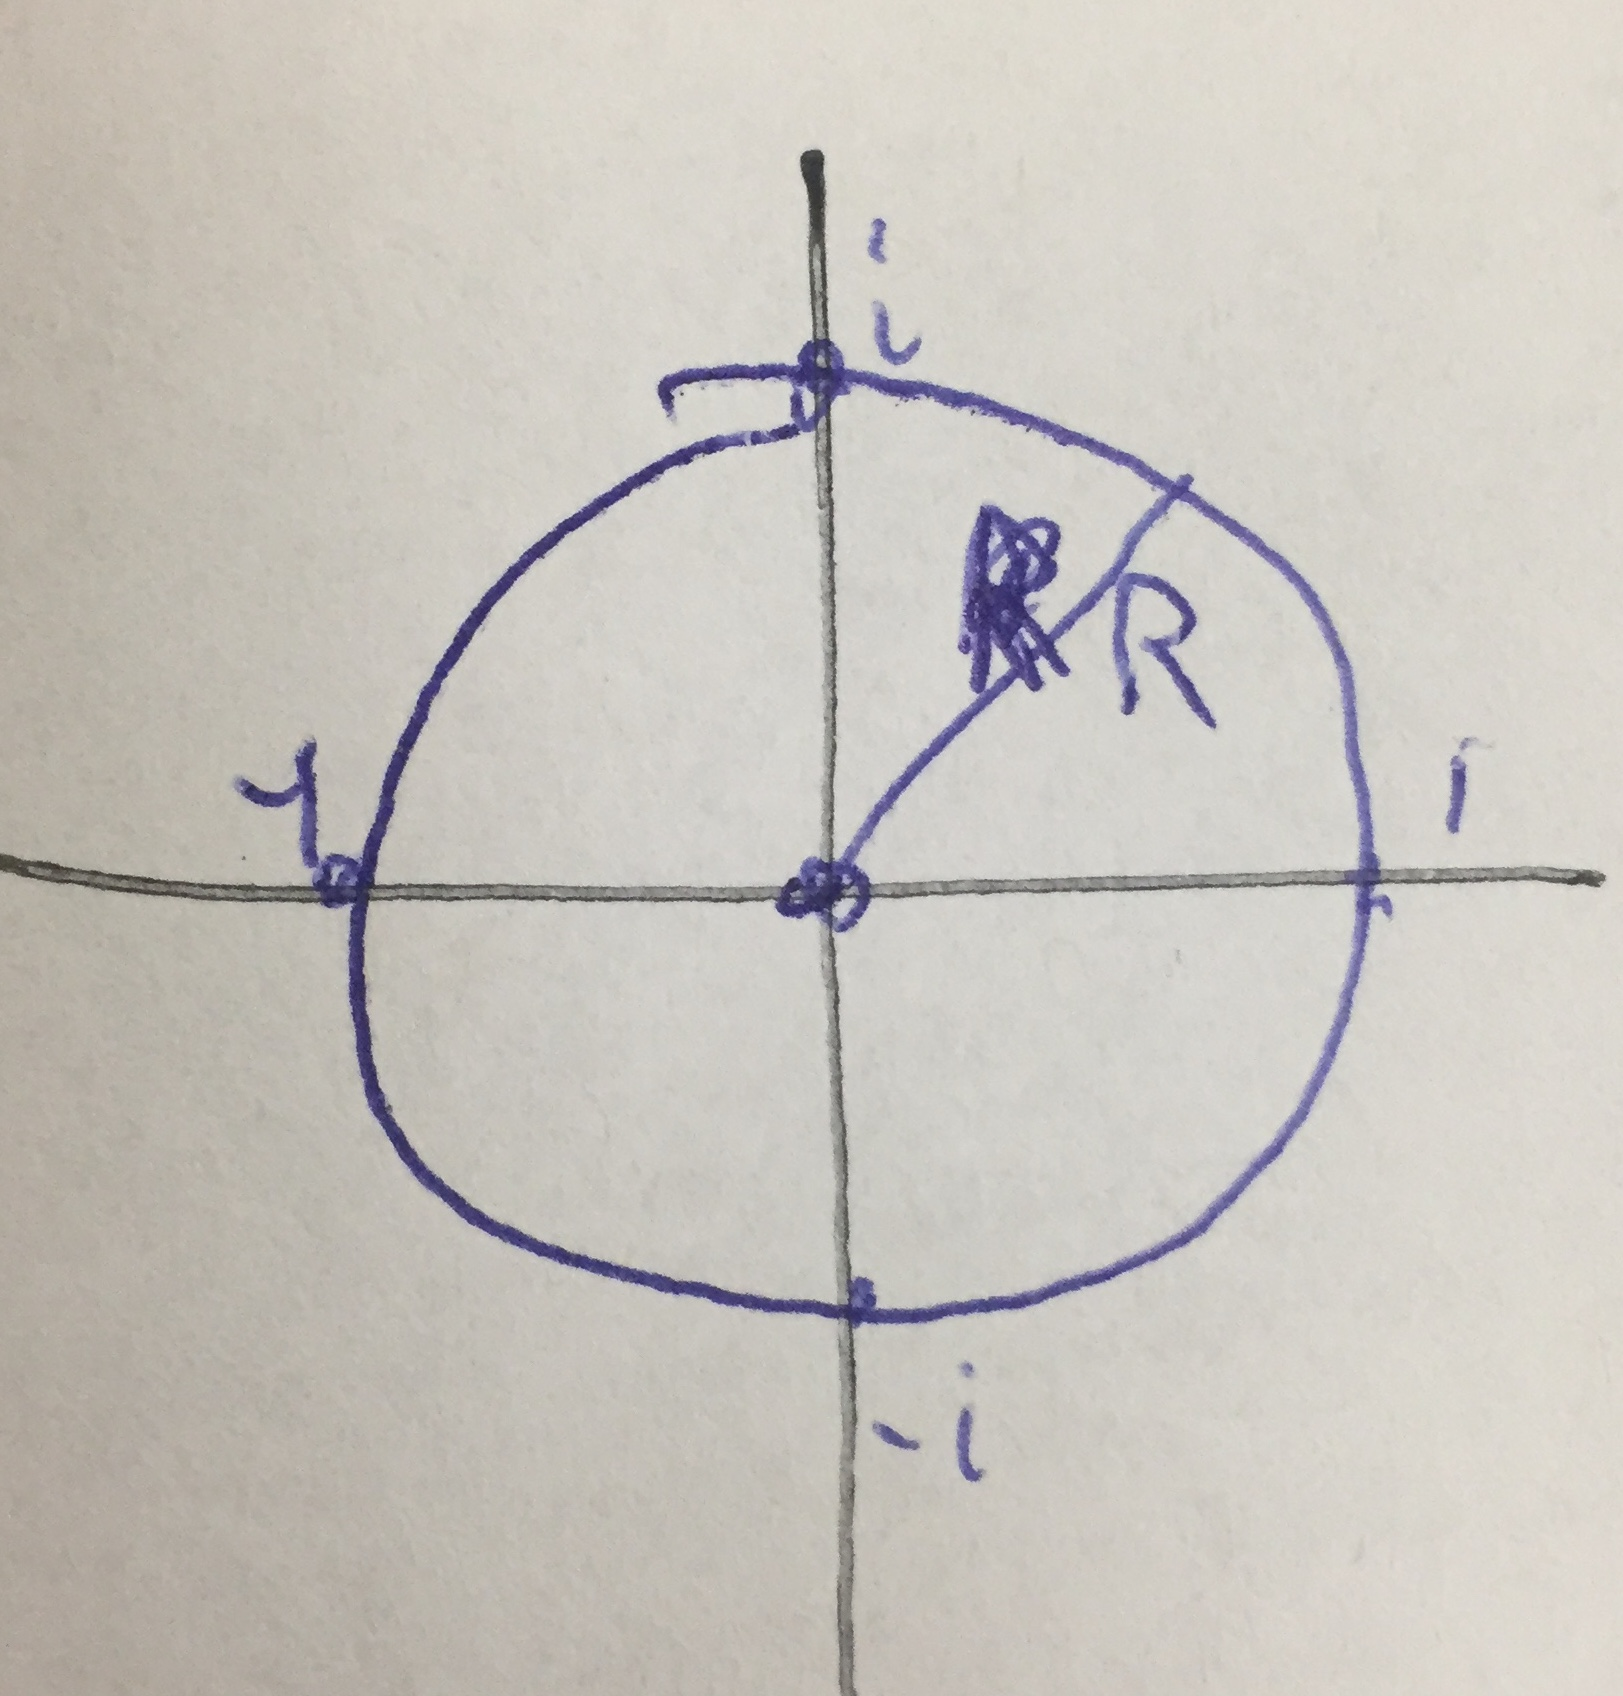
\includegraphics[scale=0.2]{Figures/circle.png}
    \caption{Make a caption. Radius of Convergence defined by r. R is length to closest singulaiity.}
\end{figure}
\be
\begin{split}
    f(1) &= e^{i\theta/2} = 1\\
    f(i) &= e^{i\pi/4} = 1\\
    f(-1) &= e^{i\pi/2} = 1\\
    f(1) &= e^{i2\pi/2} = -1\\
\end{split}
\ee
The function continuously changes about the branching point, start at 1, end at -1, the function therefore cannot be continuous. 
If you go around another time, you will get a value of 1, and so on.
This means $\sqrt{z}$ is a double-value function.


We can consider instead $\ln(z)$, and again let z=$Re^{i\theta}$, recall n=$\pm$ (1,2,3,..). 
\be
\begin{split}
    f(z) &= \ln(z) = \ln(Re^{i\theta}) = \ln(Re^{i\theta+2\pi ni}) = \ln(R) + \ln(e^{i\theta + 2\pi in})\\
    &= \ln(R) + 2\pi ni + i\theta
\end{split} 
\ee
Therefore ln is an infinite valued function (because n runs from 0 to infinity), we collect a phase each iteration
\be
\begin{split}
    \ln(1) &= 0\\
    \ln(2) &= 2\pi i\\
\end{split}
\ee

Another tyoe of singularity is an esseintail singularity, consider a Taylor expansion.
\be
f(z) = e^{1/z} =n\sum_{n=0}^\infty \frac{1}{n!}\frac{1}{z^n}
\ee
All the a$_n$ terms are $\frac{1}{n!}$ so they all exist, z=0 is an essential singularty. 

\section*{The Residue Theorem}
\be
\oint dz \quad f(z) = 2\pi i\sum_i \text{res}
\ee

Consider some function f(z) in a domain D, with isolated residues z$_1$, z$_2$, ...

\begin{figure}[H]
  \centering
    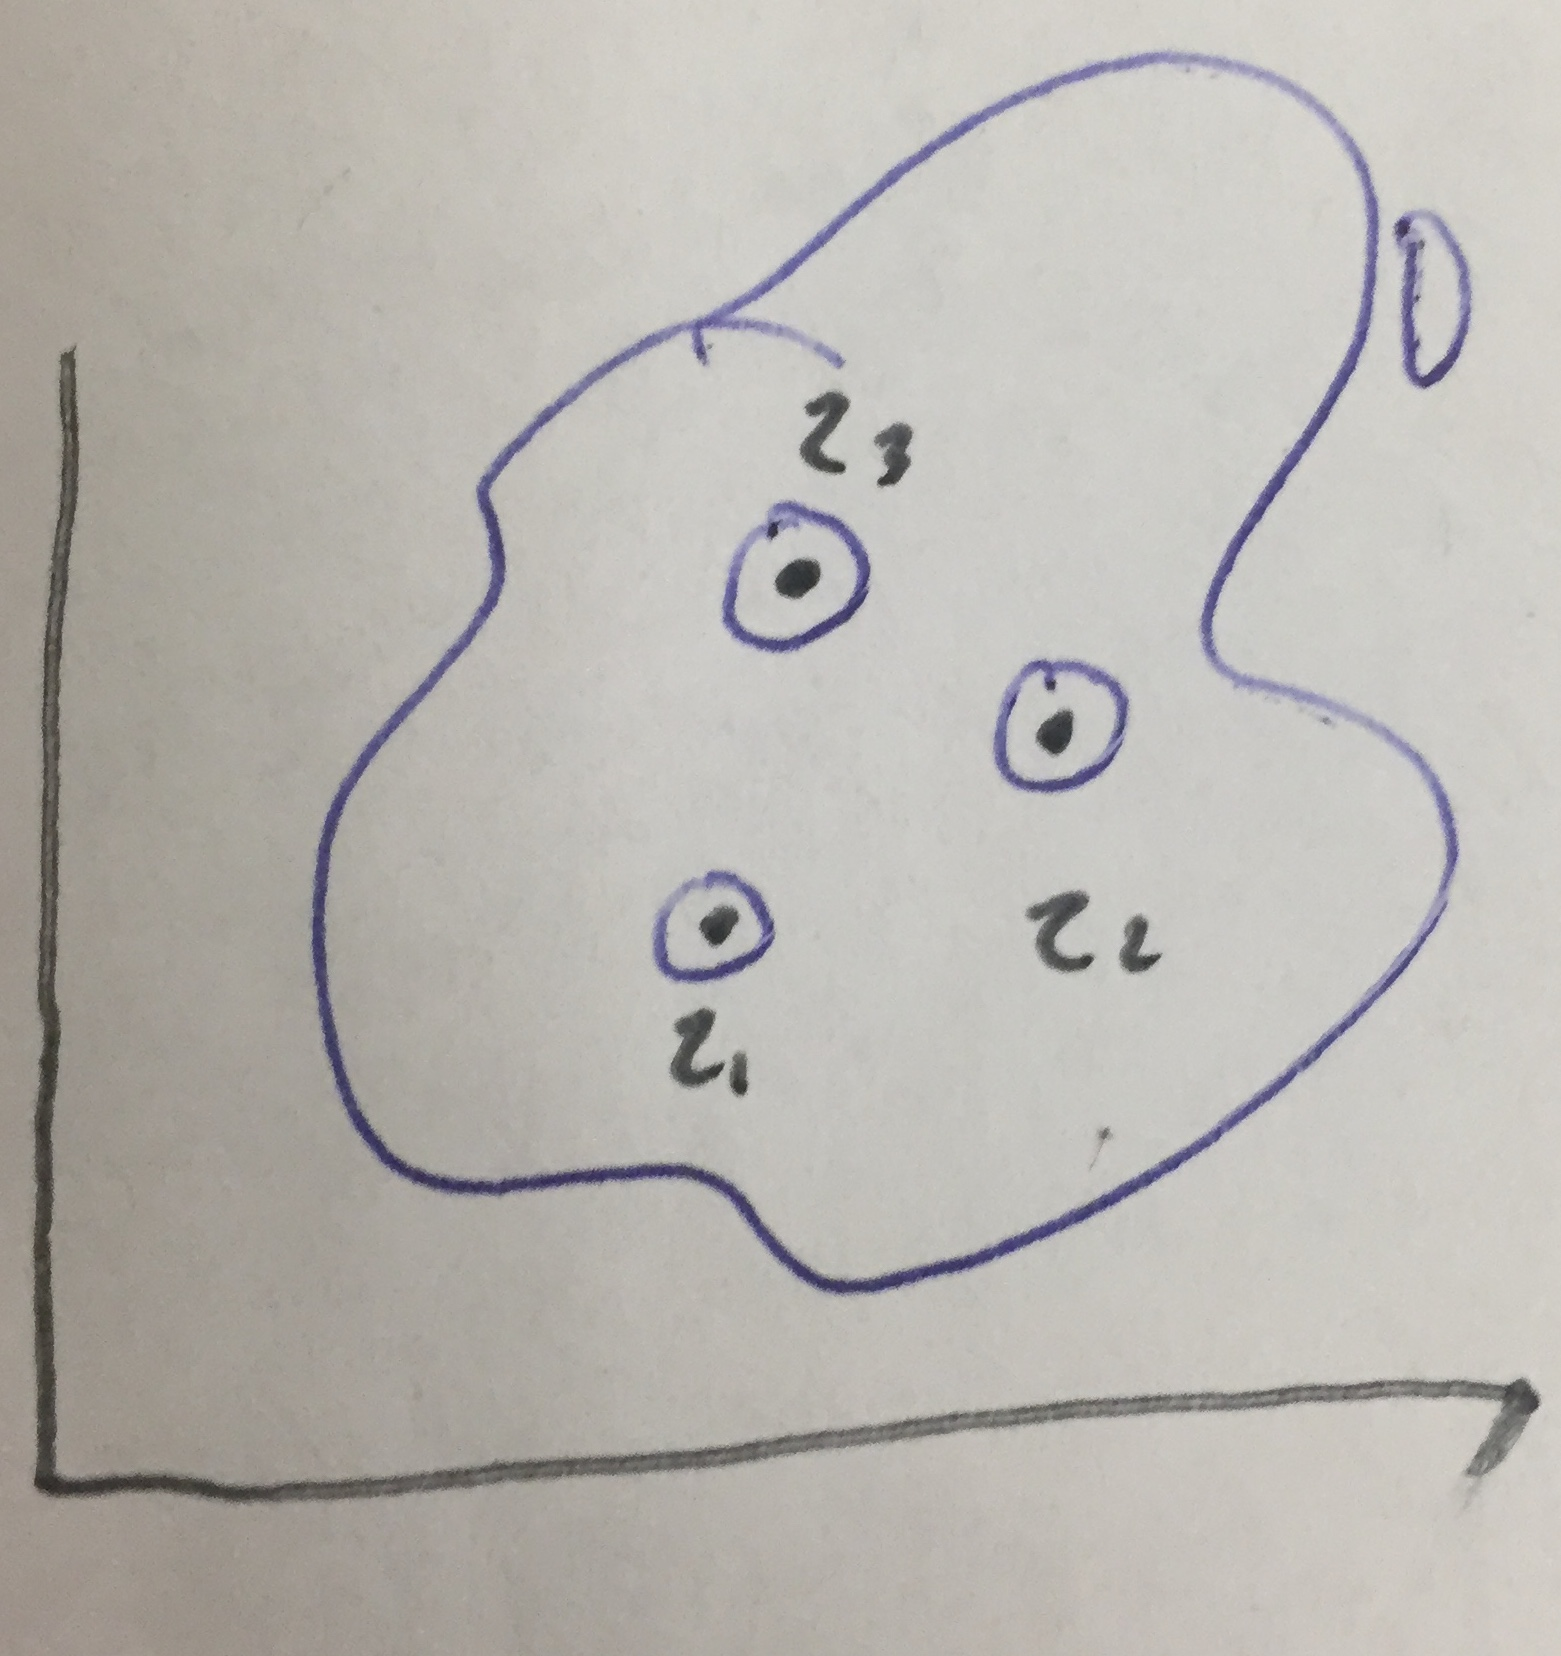
\includegraphics[scale=0.2]{Figures/res.png}
    \caption{Make a caption.isolated singularities} 
\end{figure}

If you define a contour over a set of isolated isngularities (poles) than the value of the integral is simply the values associated with the singularities through the residue theorem. 

\be
\text{residue} = \lim_{z \rightarrow z_0}{(z-z_0)} = a_1(z_0) \Rightarrow \lim_{z \rightarrow z_0}{f(z)} \frac{a_1}{(z-z_0} \Rightarrow a_1(z_0) = \text{residue}
\ee

So you need to cmpute a limit for each singularity to get the residue, and compute the integral through all of the residues. 

\subsection*{Isolated Singularities}
There own tyoe of singularity (finite power), these methods do not work forbranching points and esenitial  singularities, keep that in mind. 

As an example consider
\be
f(z) = \frac{e^z}{z^5} \Rightarrow \oint dz \quad \frac{e^z}{z^5}
\ee



\end{document}
